\documentclass[tikz,border=5pt]{standalone}
\usepackage{amsmath}
\usepackage{xcolor}
\usetikzlibrary{positioning}
\definecolor{ink}{HTML}{0F172A}
\definecolor{mutedInk}{HTML}{475569}
\definecolor{lineGray}{HTML}{CBD5E1}
\definecolor{panelGray}{HTML}{F8FAFC}
\definecolor{summaryGray}{HTML}{F1F5F9}
\definecolor{operationTeal}{HTML}{0F766E}
\definecolor{operationFill}{HTML}{ECFEFF}
\definecolor{schemaViolet}{HTML}{6D28D9}
\definecolor{schemaFill}{HTML}{F5F3FF}
\definecolor{resultGreen}{HTML}{15803D}
\definecolor{resultFill}{HTML}{F0FDF4}

\tikzset{
  state card/.style={
    draw=mutedInk,
    fill=white,
    rounded corners=1.5mm,
    line width=0.55pt,
    font=\sffamily\small,
    align=center,
    inner sep=3mm,
    text=ink
  },
  concept card/.style={
    state card,
    fill=panelGray
  },
  summary card/.style={
    state card,
    fill=summaryGray
  },
  operation card/.style={
    draw=operationTeal,
    fill=operationFill,
    rounded corners=4mm,
    line width=0.75pt,
    font=\sffamily\small\bfseries,
    align=center,
    inner xsep=4mm,
    inner ysep=2.2mm,
    text=operationTeal
  },
  schema ref/.style={
    draw=schemaViolet,
    fill=schemaFill,
    double=schemaViolet,
    double distance=1pt,
    rounded corners=1mm,
    line width=0.65pt,
    font=\sffamily\bfseries,
    inner xsep=5mm,
    inner ysep=2.5mm,
    text=schemaViolet
  },
  result card/.style={
    state card,
    draw=resultGreen,
    fill=resultFill,
    text=resultGreen,
    line width=0.75pt
  },
  bank card/.style={
    draw=schemaViolet,
    fill=white,
    rounded corners=2mm,
    line width=0.75pt,
    inner sep=4mm,
    text=ink
  },
  meta edge/.style={
    -{Stealth[length=2mm]},
    densely dashed,
    draw=mutedInk,
    line width=0.6pt
  },
  process edge/.style={
    -{Stealth[length=2.2mm]},
    draw=ink,
    line width=0.85pt
  },
  section label/.style={
    font=\sffamily\scriptsize\bfseries,
    text=mutedInk,
    align=left
  }
}


\begin{document}
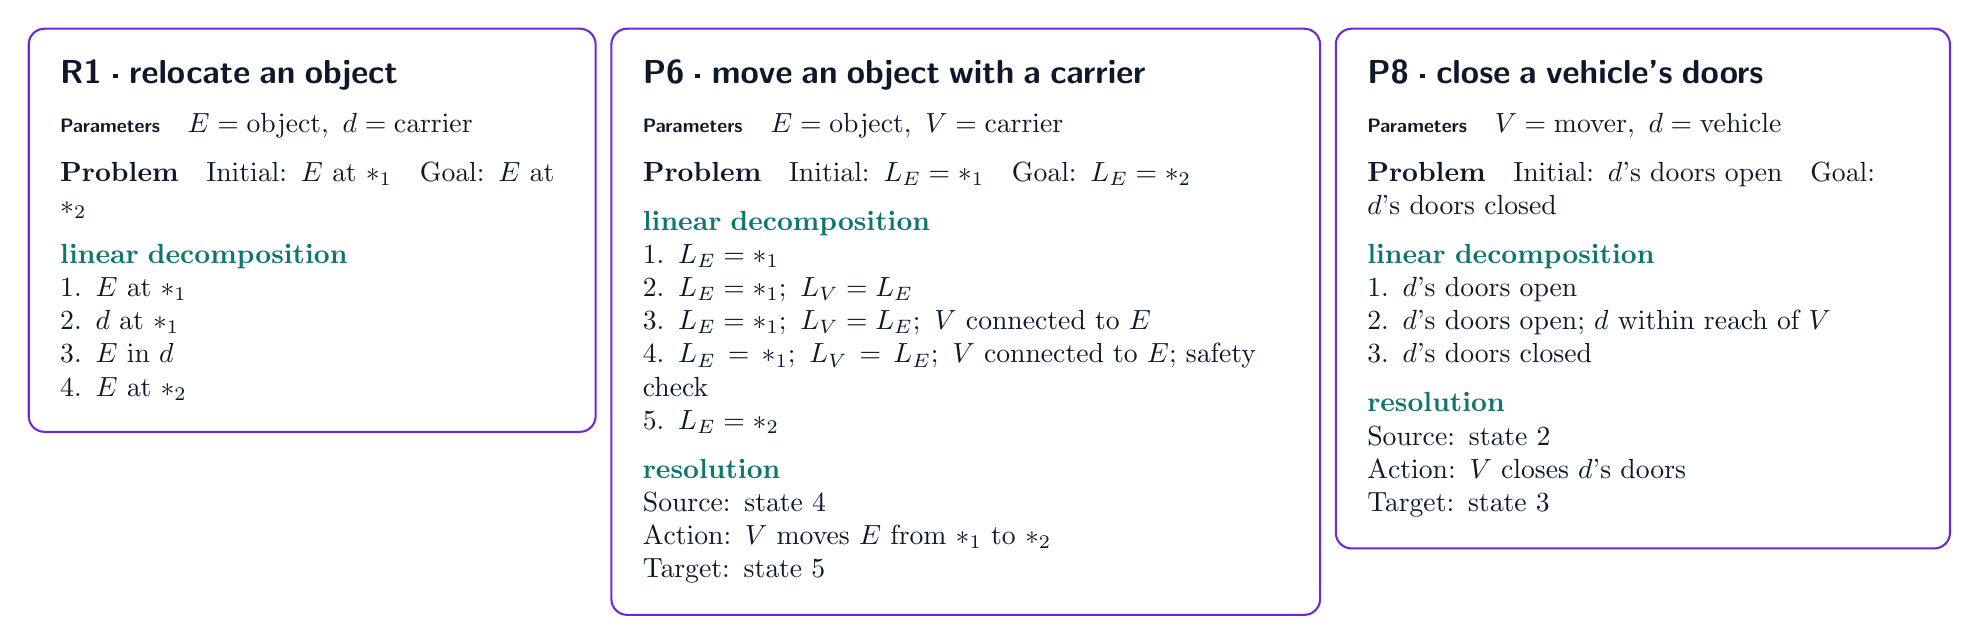
\begin{tikzpicture}
  \node[bank card,text width=64mm,anchor=north west] (r1) at (0,0) {
    {\sffamily\large\bfseries R1 · relocate an object}\\[2mm]
    {\sffamily\scriptsize\bfseries Parameters}\quad
    $E=\text{object},\ d=\text{carrier}$\\[2mm]
    \textbf{Problem}\quad
    Initial: $E$ at $*_1$\quad Goal: $E$ at $*_2$\\[2mm]
    \textcolor{operationTeal}{\textbf{linear decomposition}}\\
    1. $E$ at $*_1$\\
    2. $d$ at $*_1$\\
    3. $E$ in $d$\\
    4. $E$ at $*_2$
  };

  \node[bank card,text width=82mm,anchor=north west] (p6) at (7.4,0) {
    {\sffamily\large\bfseries P6 · move an object with a carrier}\\[2mm]
    {\sffamily\scriptsize\bfseries Parameters}\quad
    $E=\text{object},\ V=\text{carrier}$\\[2mm]
    \textbf{Problem}\quad
    Initial: $L_E=*_1$\quad Goal: $L_E=*_2$\\[2mm]
    \textcolor{operationTeal}{\textbf{linear decomposition}}\\
    1. $L_E=*_1$\\
    2. $L_E=*_1;\ L_V=L_E$\\
    3. $L_E=*_1;\ L_V=L_E;\ V$ connected to $E$\\
    4. $L_E=*_1;\ L_V=L_E;\ V$ connected to $E$; safety check\\
    5. $L_E=*_2$\\[2mm]
    \textcolor{operationTeal}{\textbf{resolution}}\\
    Source: state 4\\
    Action: $V$ moves $E$ from $*_1$ to $*_2$\\
    Target: state 5
  };

  \node[bank card,text width=70mm,anchor=north west] (p8) at (16.6,0) {
    {\sffamily\large\bfseries P8 · close a vehicle's doors}\\[2mm]
    {\sffamily\scriptsize\bfseries Parameters}\quad
    $V=\text{mover},\ d=\text{vehicle}$\\[2mm]
    \textbf{Problem}\quad
    Initial: $d$'s doors open\quad Goal: $d$'s doors closed\\[2mm]
    \textcolor{operationTeal}{\textbf{linear decomposition}}\\
    1. $d$'s doors open\\
    2. $d$'s doors open; $d$ within reach of $V$\\
    3. $d$'s doors closed\\[2mm]
    \textcolor{operationTeal}{\textbf{resolution}}\\
    Source: state 2\\
    Action: $V$ closes $d$'s doors\\
    Target: state 3
  };
\end{tikzpicture}
\end{document}
